%% paper_template.tex is a modification of:
%% bare_conf.tex 
%% V1.2
%% 2002/11/18
%% by Michael Shell
%% mshell@ece.gatech.edu
%% 
%% This is a skeleton file demonstrating the use of IEEEtran.cls 
%% (requires IEEEtran.cls version 1.6b or later) with an IEEE conference paper.
%% 
%% Support sites:
%% http://www.ieee.org
%% and/or
%% http://www.ctan.org/tex-archive/macros/latex/contrib/supported/IEEEtran/ 
%%
%% This code is offered as-is - no warranty - user assumes all risk.
%% Free to use, distribute and modify.

% *** Authors should verify (and, if needed, correct) their LaTeX system  ***
% *** with the testflow diagnostic prior to trusting their LaTeX platform ***
% *** with production work. IEEE's font choices can trigger bugs that do  ***
% *** not appear when using other class files.                            ***
% Testflow can be obtained at:
% http://www.ctan.org/tex-archive/macros/latex/contrib/supported/IEEEtran/testflow


% Note that the a4paper option is mainly intended so that authors in
% countries using A4 can easily print to A4 and see how their papers will
% look in print. Authors are encouraged to use U.S. letter paper when 
% submitting to IEEE. Use the testflow package mentioned above to verify
% correct handling of both paper sizes by the author's LaTeX system.
%
% Also note that the "draftcls" or "draftclsnofoot", not "draft", option
% should be used if it is desired that the figures are to be displayed in
% draft mode.
%
% This paper can be formatted using the % (instead of conference) mode.
%++++++++++++++++++++++++++++++++++++++++++++++++++++++
%\documentclass[conference]{IEEEims} % Modified for MTT-IMS
%\documentclass[conference]{IMSTemplate}


\documentclass[conference]{IEEEtran}
%++++++++++++++++++++++++++++++++++++++++++++++++++++++
% If the IEEEtran.cls has not been installed into the LaTeX system files, 
% manually specify the path to it:
% \documentclass[conference]{../sty/IEEEtran} 


% some very useful LaTeX packages include:

%\usepackage{cite}      % Written by Donald Arseneau
                        % V1.6 and later of IEEEtran pre-defines the format
                        % of the cite.sty package \cite{} output to follow
                        % that of IEEE. Loading the cite package will
                        % result in citation numbers being automatically
                        % sorted and properly "ranged". i.e.,
                        % [1], [9], [2], [7], [5], [6]
                        % (without using cite.sty)
                        % will become:
                        % [1], [2], [5]--[7], [9] (using cite.sty)
                        % cite.sty's \cite will automatically add leading
                        % space, if needed. Use cite.sty's noadjust option
                        % (cite.sty V3.8 and later) if you want to turn this
                        % off. cite.sty is already installed on most LaTeX
                        % systems. The latest version can be obtained at:
                        % http://www.ctan.org/tex-archive/macros/latex/contrib/supported/cite/

%\usepackage{graphicx}  % Written by David Carlisle and Sebastian Rahtz
                        % Required if you want graphics, photos, etc.
                        % graphicx.sty is already installed on most LaTeX
                        % systems. The latest version and documentation can
                        % be obtained at:
                        % http://www.ctan.org/tex-archive/macros/latex/required/graphics/
                        % Another good source of documentation is "Using
                        % Imported Graphics in LaTeX2e" by Keith Reckdahl
                        % which can be found as esplatex.ps and epslatex.pdf
                        % at: http://www.ctan.org/tex-archive/info/
% NOTE: for dual use with latex and pdflatex, instead load graphicx like:
%\ifx\pdfoutput\undefined
%\usepackage{graphicx}
%\else
%\usepackage[pdftex]{graphicx}
%\fi
%+++++++++++++++++++++++++++++++++++++++++++
% Added to commands
\input epsf
\usepackage{graphicx}
\usepackage[]{algorithm2e}
\usepackage{graphicx}
\usepackage{enumitem}
\usepackage{tabularx}
\usepackage{multirow}
\usepackage{longtable}
\usepackage{multicol}
\usepackage{lipsum}
\usepackage{floatrow}
\usepackage{tikz}
\usetikzlibrary{shapes.geometric, arrows}
\usepackage{multirow}
\renewcommand{\labelitemii}{$\star$}
\usepackage{xcolor}
\usepackage[font=small,labelfont=bf,tableposition=top]{caption}
\usepackage[official,right]{eurosym}
\usepackage{rotating}

%\usepackage{pdflscape}

\usepackage{afterpage}
\usepackage{amssymb}

\usepackage{amsmath}
\usepackage{amsfonts}


\usepackage{hyperref}
\usepackage{graphicx}
\usepackage{floatrow}
%\usepackage[a4paper,left=15mm,right=15mm, top=1cm, bottom=2cm]{geometry}% http://ctan.org/pkg/geometry
\usepackage{blindtext}

\usepackage{tikz}
\usetikzlibrary{shapes.geometric, arrows}
\usepackage{multirow}

\usepackage{xcolor}
\hypersetup{
    colorlinks,
    linkcolor=blue,
    citecolor=blue,
    urlcolor=blue
}
\usepackage[font=small,labelfont=bf,tableposition=top]{caption}
\usepackage[official,right]{eurosym}
\usepackage{rotating}

\newcount\n
\n=0
\def\tablebody{}
\makeatletter
\loop\ifnum\n<50
    \advance\n by1
    \protected@edef\tablebody{\tablebody
            \textbf{\number\n.}& shortText & longlonglonglonglong text
            longlonglonglonglong text
            \tabularnewline
n    }
\repeat
\makeatother
%+++++++++++++++++++++++++++++++++++++++++++
% However, be warned that pdflatex will require graphics to be in PDF
% (not EPS) format and will preclude the use of PostScript based LaTeX
% packages such as psfrag.sty and pstricks.sty. IEEE conferences typically
% allow PDF graphics (and hence pdfLaTeX). However, IEEE journals do not
% (yet) allow image formats other than EPS or TIFF. Therefore, authors of
% journal papers should use traditional LaTeX with EPS graphics.
%
% The path(s) to the graphics files can also be declared: e.g.,
% \graphicspath{{../eps/}{../ps/}}
% if the graphics files are not located in the same directory as the
% .tex file. This can be done in each branch of the conditional above
% (after graphicx is loaded) to handle the EPS and PDF cases separately.
% In this way, full path information will not have to be specified in
% each \includegraphics command.
%
% Note that, when switching from latex to pdflatex and vice-versa, the new
% compiler will have to be run twice to clear some warnings.


%\usepackage{psfrag}    % Written by Craig Barratt, Michael C. Grant,
                        % and David Carlisle
                        % This package allows you to substitute LaTeX
                        % commands for text in imported EPS graphic files.
                        % In this way, LaTeX symbols can be placed into
                        % graphics that have been generated by other
                        % applications. You must use latex->dvips->ps2pdf
                        % workflow (not direct pdf output from pdflatex) if
                        % you wish to use this capability because it works
                        % via some PostScript tricks. Alternatively, the
                        % graphics could be processed as separate files via
                        % psfrag and dvips, then converted to PDF for
                        % inclusion in the main file which uses pdflatex.
                        % Docs are in "The PSfrag System" by Michael C. Grant
                        % and David Carlisle. There is also some information 
                        % about using psfrag in "Using Imported Graphics in
                        % LaTeX2e" by Keith Reckdahl which documents the
                        % graphicx package (see above). The psfrag package
                        % and documentation can be obtained at:
                        % http://www.ctan.org/tex-archive/macros/latex/contrib/supported/psfrag/

%\usepackage{subfigure} % Written by Steven Douglas Cochran
                        % This package makes it easy to put subfigures
                        % in your figures. i.e., "figure 1a and 1b"
                        % Docs are in "Using Imported Graphics in LaTeX2e"
                        % by Keith Reckdahl which also documents the graphicx
                        % package (see above). subfigure.sty is already
                        % installed on most LaTeX systems. The latest version
                        % and documentation can be obtained at:
                        % http://www.ctan.org/tex-archive/macros/latex/contrib/supported/subfigure/

%\usepackage{url}       % Written by Donald Arseneau
                        % Provides better support for handling and breaking
                        % URLs. url.sty is already installed on most LaTeX
                        % systems. The latest version can be obtained at:
                        % http://www.ctan.org/tex-archive/macros/latex/contrib/other/misc/
                        % Read the url.sty source comments for usage information.

%\usepackage{stfloats}  % Written by Sigitas Tolusis
                        % Gives LaTeX2e the ability to do double column
                        % floats at the bottom of the page as well as the top.
                        % (e.g., "\begin{figure*}[!b]" is not normally
                        % possible in LaTeX2e). This is an invasive package
                        % which rewrites many portions of the LaTeX2e output
                        % routines. It may not work with other packages that
                        % modify the LaTeX2e output routine and/or with other
                        % versions of LaTeX. The latest version and
                        % documentation can be obtained at:
                        % http://www.ctan.org/tex-archive/macros/latex/contrib/supported/sttools/
                        % Documentation is contained in the stfloats.sty
                        % comments as well as in the presfull.pdf file.
                        % Do not use the stfloats baselinefloat ability as
                        % IEEE does not allow \baselineskip to stretch.
                        % Authors submitting work to the IEEE should note
                        % that IEEE rarely uses double column equations and
                        % that authors should try to avoid such use.
                        % Do not be tempted to use the cuted.sty or
                        % midfloat.sty package (by the same author) as IEEE
                        % does not format its papers in such ways.

%\usepackage{amsmath}   % From the American Mathematical Society
                        % A popular package that provides many helpful commands
                        % for dealing with mathematics. Note that the AMSmath
                        % package sets \interdisplaylinepenalty to 10000 thus
                        % preventing page breaks from occurring within multiline
                        % equations. Use:
%\interdisplaylinepenalty=2500
                        % after loading amsmath to restore such page breaks
                        % as IEEEtran.cls normally does. amsmath.sty is already
                        % installed on most LaTeX systems. The latest version
                        % and documentation can be obtained at:
                        % http://www.ctan.org/tex-archive/macros/latex/required/amslatex/math/



% Other popular packages for formatting tables and equations include:

%\usepackage{array}
% Frank Mittelbach's and David Carlisle's array.sty which improves the
% LaTeX2e array and tabular environments to provide better appearances and
% additional user controls. array.sty is already installed on most systems.
% The latest version and documentation can be obtained at:
% http://www.ctan.org/tex-archive/macros/latex/required/tools/

% Mark Wooding's extremely powerful MDW tools, especially mdwmath.sty and
% mdwtab.sty which are used to format equations and tables, respectively.
% The MDWtools set is already installed on most LaTeX systems. The lastest
% version and documentation is available at:
% http://www.ctan.org/tex-archive/macros/latex/contrib/supported/mdwtools/


% V1.6 of IEEEtran contains the IEEEeqnarray family of commands that can
% be used to generate multiline equations as well as matrices, tables, etc.


% Also of notable interest:

% Scott Pakin's eqparbox package for creating (automatically sized) equal
% width boxes. Available:
% http://www.ctan.org/tex-archive/macros/latex/contrib/supported/eqparbox/



% Notes on hyperref:
% IEEEtran.cls attempts to be compliant with the hyperref package, written
% by Heiko Oberdiek and Sebastian Rahtz, which provides hyperlinks within
% a document as well as an index for PDF files (produced via pdflatex).
% However, it is a tad difficult to properly interface LaTeX classes and
% packages with this (necessarily) complex and invasive package. It is
% recommended that hyperref not be used for work that is to be submitted
% to the IEEE. Users who wish to use hyperref *must* ensure that their
% hyperref version is 6.72u or later *and* IEEEtran.cls is version 1.6b 
% or later. The latest version of hyperref can be obtained at:
%
% http://www.ctan.org/tex-archive/macros/latex/contrib/supported/hyperref/
%
% Also, be aware that cite.sty (as of version 3.9, 11/2001) and hyperref.sty
% (as of version 6.72t, 2002/07/25) do not work optimally together.
% To mediate the differences between these two packages, IEEEtran.cls, as
% of v1.6b, predefines a command that fools hyperref into thinking that
% the natbib package is being used - causing it not to modify the existing
% citation commands, and allowing cite.sty to operate as normal. However,
% as a result, citation numbers will not be hyperlinked. Another side effect
% of this approach is that the natbib.sty package will not properly load
% under IEEEtran.cls. However, current versions of natbib are not capable
% of compressing and sorting citation numbers in IEEE's style - so this
% should not be an issue. If, for some strange reason, the user wants to
% load natbib.sty under IEEEtran.cls, the following code must be placed
% before natbib.sty can be loaded:
%
% \makeatletter
% \let\NAT@parse\undefined
% \makeatother
%
% Hyperref should be loaded differently depending on whether pdflatex
% or traditional latex is being used:
%
%\ifx\pdfoutput\undefined
%\usepackage[hypertex]{hyperref}
%\else
%\usepackage[pdftex,hypertexnames=false]{hyperref}
%\fi
%
% Pdflatex produces superior hyperref results and is the recommended
% compiler for such use.



% *** Do not adjust lengths that control margins, column widths, etc. ***
% *** Do not use packages that alter fonts (such as pslatex).         ***
% There should be no need to do such things with IEEEtran.cls V1.6 and later.


% correct bad hyphenation here
\hyphenation{op-tical net-works semi-conduc-tor IEEEtran}
\begin{document}

% paper title
%\title{Submission Format for IMS2014 (Title in 24-point Times font)}
% If the \LARGE is deleted, the title font defaults to  24-point.
% Actually, 
% the \LARGE sets the title at 17 pt, which is close enough to 18-point.
%+++++++++++++++++++++++++++++++++++++++++++
\title{\LARGE Vulnerabilities Evolution: An Empirical Study of Static Analysis Tools Capabilities}



%\author{\IEEEauthorblockN{Bushra Aloraini}
%\IEEEauthorblockA{David R. Cheriton School of Computer Science \\
%University of Waterloo\\
%Waterloo, ON, Canada\\
%balorain@uwaterloo.ca}

%\and
%\IEEEauthorblockN{Meiyappan Nagappan}
%\IEEEauthorblockA{David R. Cheriton School of Computer Science \\
%University of Waterloo\\
%Waterloo, ON, Canada\\
%mei.nagappan@uwaterloo.ca}
%}


% make the title area
\maketitle

\begin{abstract}
This paper aims to study and understand 
the evolution of software vulnerabilities 
and the capability of static analysis tools 
in software repositories. 
In this study, we aim at studying the evolution of vulnerabilities 
detected by six static analysis tools (SATs). 
Instead of using crafted test cases, 
we will be examined large and real 400 popular C++ project repositories. 
The main goal of this paper is to 
investigate the evolution of different types of vulnerabilities 
and discuses the reasons for vulnerability removals. 
The study is performed by using framework that 
traces source code lines across different commits.

  % Instead of running static analysis tools against test cases to measure the efficiency and capability, we want to evaluate such static analysis tools against real applications. That is because real applications contain real vulnerabilities and not vulnerabilities that were built based on a specific assumption in which static analysis tools know those kind of assumed vulnerabilities (and potentially built based on that to detect those assumed vulnerabilities). Indeed, a study by the National Security Agency (NSA) \cite{nsa2011} has emphasized the importance of evaluating static analysis tools against real applications to more precisely predict the frequencies of vulnerabilities outside of controlled studies.
\end{abstract}

\IEEEoverridecommandlockouts

\IEEEpeerreviewmaketitle

%\section{Introduction}
Cyberattack has became a significant universal threat that poses a very serious economic loss, reputational damage, and could expose organizations to legal consequences, such as negligence claims and the failure to meet contractual obligations \cite{mcafee2014}. It is anticipated that upcoming years will witness more cyberattacks due to the emerging of the Internet of Things technologies which could influence everyone \cite{securitynewsdesk2017}. Hence, cybersecurity has become a significant concern. 

Despite that there are several security defense solutions are introduced ever since, however building secure software in the first place is the first line of defense. In fact, software security vulnerabilities are estimated to be one of the most used attack vector by attacker rated as 60-90\% of all attacks \cite{heimdalsecurity2016}. Therefore, software testing to ensure software security has attracted much attention in software engineering community. Static analysis is one way used during software testing to find security vulnerabilities early during the coding phase. This leads to cost saving which is a key benefit of static analysis tools \cite{soni2006defect}.  

Static analysis tools are used to analyses the source or binary code of the program without executing it. These tools could provide various insights into the program's code, such as analyzing its structures and dependencies, providing code metrics, detecting bugs, etc. In this paper, we are interested in studying static analysis tools that detect one of the most dangerous and frequent type of venerabilities, buffer overflow \cite{Cowan2003}.  There are multiple static analysis methods and tools that were introduced to detect such vulnerability during coding phase. These different static analysis tools adopt different analysis methods to detect buffer overflow. In fact , different static analysis tools that target buffer overflow vulnerabilities could be able to detect some variants of buffer overflow vulnerabilities but not others.

In this study, we want to study the capabilities and the effectiveness of static analysis tools that could detect buffer overflow vulnerabilities in C++. However, instead of running static analysis tools against test cases to measure the efficiency and capability, we want to evaluate such static analysis tools against real applications. That is because real applications contain real vulnerabilities and not vulnerabilities that were built based on a specific assumption in which static analysis tools know those kind of assumed vulnerabilities (and potentially built based on that to detect those assumed vulnerabilities). Indeed, a study by the National Security Agency (NSA) \cite{nsa2011} has emphasized the importance of evaluating static analysis tools against real applications to more  precisely predict the frequencies of bugs outside of controlled studies.

Large repositories could provide a great opportunity in this matter. Large repositories maintain rich historical data, such as the code changes, bugs and issues history,  how software evolved over time, etc. Buffer overflow could potentially introduce to the software at a certain time, then it could be removed  at another time. In fact, studying bugs at large repository not only gives us the true story about the bug but also it could provide more information regarding that discovered bugs such as bug frequency, pattern, and age.  

Therefore, our study focus on studying the effectiveness of static analysis tools by utilizing information provided by large repositories. In particular, we want to see how efficient static analysis tools are in detecting such vulnerability, and are these static analysis tools able to detect real vulnerabilities.  We measure the efficiency in terms of false positive rate, the precision, and running time.  Also, we want to investigate whether buffer overflow bugs have a specific pattern that leads to be detected by static analysis tools. Moreover, we want to study how these detected vulnerabilities evolved over time and how frequent are they. So, we will investigate that by examining the following RQs: 
\section{Data extraction} {{{2
to extract data necessary for the analysis 
of source code vulnerability evolution. 
The data extraction process consists of the sequence of five steps:

\begin{itemize}
\item  \textbf{Step 1: snapshots extraction}
As we are working on GitHub repositories, 
so we will be identifying two snapshots: 
one in 2012 and the other in 2017. 

\item \textbf{Step 2: identification of vulnerable source code lines}  
We will be running all SATs on 2012 and 2017 versions, 
however we are interested in all vulnerabilities that 
were flagged in 2012 and removed from the code in 2017. 
This analysis will help us to identify the set of source code lines
that contain warnings on both 2012 and 2017 versions. 
The output of this step is, for each snapshot, 
the list of vulnerable source code lines with
a vulnerability description as extracted by the tool, 
and a vulnerability classification according to the used vulnerabilities taxonomy. 

\item \textbf{Step 3: differences identification and line tracing} 
To analyze the evolution of vulnerable source code lines over snapshots, 
we need to identify in each tested file the addition of new lines, 
in the removal of existing lines, and the change of existing lines. 
Therefore, we will be using tracing tools such as ldiff tool. 

\item \textbf{Step 4: determining vulnerability changes among snapshots}
In this research question, we could identify false positive and true positive warnings, 
and this by considering the following cases:
	Any vulnerability warning that was reported in 2012 and 2017 
    will be consider to be false positives.
	Any vulnerability warning that was reported in 2012 but not 2017 
    will be considered for further analysis: 
    1- when  a source code line containing a vulnerability was removed, 
    2- the source code line has changed, 
    or 3-  the source code line  has not been changed but a change occurred somewhere else.

\item \textbf{Step 5: analyzing documentation of vulnerability removal/ disappear} 
To better understand in what context a vulnerability was removed or disappeared,
we will be using automatic analysis on all the commit messages
that indicate vulnerability fix following \cite{mockus2000identifying} method. 
\end{itemize}


\begin{itemize}
\item \textbf{RQ1: How effective the studied static analysis tools are?}
We  measure the effective of he studied static analysis tools in terms of precision, false positive rate, running time. We found that RATS outperform other tools regarding the running time. While Flawfinder found to be more precise and has less false positive rate, though Cppcheck did not produced any buffer overflow warning.
\item \textbf{RQ2: How true positive vulnerabilities evolve over time?}
We focus here on vulnerabilities age. We found that  most of the true positive vulnerabilities were detected and deleted in less than 6 months period of time. However, there were some vulnerabilities that up to aged 71 months, about 5 years and 9 months, and then finally removed. The result need further investigation using more advanced static analysis tools to confirm this finding.

\item \textbf{RQ3: What are the patterns of buffer overflow bugs in which they were detected by static analysis tools?}
We focus here on vulnerabilities frequency. We found that calling potentially dangerous functions to be the most frequent pattern that occurred in true positive warnings. Other categories that happed frequently as well are fixed buffer size and unsensitized input from untrusted sources
\end{itemize}


We believe that conducting this study will gave us a better understanding of the pattern of emerging buffer overflow vulnerabilities. In addition, at the end of this study we will able to recognize which static analysis methods perform better. Thus, we will be able to build a better a tool to discover such vulnerability.

%\section{Related Work}
Some studies have evaluated the use of static analysis tools for buffer overflow detection  \cite{Zitser2004}  \cite{Torri2010}  \cite{Kratkiewicz2005}. All these mentioned studies were conducted on a few number of programs that have small size.  For instance, Zitser et al. have conducted the study on three open source programs: BIND, WU-FTPD, and Sendmail that contain 14 exploitable buffer overflow vulnerabilities to test 5 open source static analysis tools. While Torri et al. conducted similar study but it was generalized for multiple vulnerabilities types. The study was conducted on 5 programs that include 17 buffer overflow vulnerabilities in total. Kratkiew et al. have evaluated 291 small C program test cases.  However, our study  is the first empirical study aims to understand buffer overflow vulnerabilities by utilizing information that is maintained in large repositories. Our study, included mining 40 large projects with their commits. Also, all previous mentioned studies have been conducted on test cases, however we aim to evaluate real program and not test cases. In addition, all above mentioned studies were conducted on C language, but our study aims at studying static analysis tools that target both C++. 

In addition to evaluate the efficiency of static analysis tools, our study also is the first study that aims to extract the pattern and the age of true positive vulnerabilities. In addition, our goal is to uncover the underlying technique of static analysis tools that detect real buffer overflow vulnerabilities. Table \ref{RealtedWork} shows the difference between our research and the previous research work that were conducted in studying the effectiveness of static analysis tools. 



\begin{table} [h!]
\centering
\scriptsize
%\resizebox{\textwidth}{!}{%
\caption{\# The difference between this study and the previous research work that were conducted in studying the effectiveness of static analysis tools to detect buffer overflow}
\label{RealtedWork}
\scriptsize
\centering
%\hspace*{-1cm}
%\fontsize{6pt}{9pt}
\begin{tabular}{||p{2cm} |p{1cm} p{1cm} p{1cm} p{1cm}||}
%\begin{tabular}{|l|l|l|l|l|l|}
%\begin{tabular}{|p|c|c|c|c|c|}

\hline
\textbf{Research} &  \textbf{Zitser et. al}  \cite{Zitser2004}  & \textbf{Torri et. al} \cite{Torri2010} & \textbf{Kratkiew et. al} \cite{Kratkiewicz2005}&
\textbf{This study} \\  [0.5ex]
\hline\hline
Size of Projects & Small & Small & Small &  Large 
\\  
Number of Projects & 3&5&291& 40  +cmts 
\\ 
 Number of Tools & 5 & 7&5 &3
\\  
Language & C &C&C&C++
\\  
Type &  Test case & Test case & Test case & Real
\\  

History & No& No& No & Yes
\\ \hline

\end{tabular}	
\end{table}


%\section{Methods}
\subsection{Data Collection}
our study depends on three types of data: (1) Large repositories that include C++ source code which could contain buffer overflow vulnerabilities, (2) Static analysis tools that could analyze the source code, and (3) Vulnerability reports that are generated from running static analysis tools against the source code of the repositories. In the following section, a detailed description about each conducted step.
\newline
\subsubsection{\textbf{Selecting Projects}}
Our goal was to study the effectiveness of static analysis tools through studying the historical data of large repositories. Therefore, GitHub was chosen to conduct such an analysis. We used RepoReapers dataset \cite{Reporeapers2016} to retrieve our dataset. As we wanted to focus on C++ projects, we filtered RepoReapers dataset to include only projects that are written in C++. Since our analysis depends on the historical data in these large repertoires, we needed to mine projects that have adequately long historical data. Thus, we selected projects in RepoReapers dataset that have the most stars, which indicates the projects popularity. As those projects are more likely to be more active and thus have more number of commits. Then, we ordered RepoReapers dataset by the highest number of stars, then we selected the top 10,000. After that, we randomly selected 400 projects from the 10,000 list. When we mined the chosen repositories from GitHub, we applied some criteria to ensure the robustness of our dataset. For instance, we built a tool to ensure that retrieved projects are indeed C++ projects. We found that 27 of mined projects are not C++ projects and thus we removed them from our dataset; and selected new ones randomly from the 10,000 list. In addition, we excluded projects with fewer than 40 commits, we found that 17 projects have less than 40 commits which were excluded then. Also, all mined projects were tested to see whether they adopt cmake build system, as we planed to expand our analysis to test more advanced static analysis tools that analyze projects based on that build system. We found 270 projects are not adopting cmake build, thus we continently cloned projects from the 10,000 list to construct our dataset. In all cases that we needed to clone new project from the 10,000 list, we ensured that new selected new one that are not included in our 400 list. For this study, we run our analysis against only 40 projects that were chosen randomly.
\newline

\subsubsection{\textbf{Gathering Static Analysis Tools}}
We gathered three open source static analysis tools that discover buffer overflow. Our study tests the following tools that support C++:  Cppcheck \cite{Torri2010}, Flawfinder \cite{Torri2010}, and RATS \cite{Torri2010}.  Table \ref{C++SAT} summarizes all tested tools and their versions. 


\begin{table}[ht]
\centering
\scriptsize
\caption{The Studied free and open source static analysis tools that detect buffer overflow in C++}
\label{C++SAT}
\begin{tabular}{||p{1.5cm}|p{1cm} p{2.6cm}p{1.2cm}||}
\hline
 \textbf{Tool Name} &  \textbf{Language} &\textbf{Inference Algorithm} &  \textbf{Version Number}\\

\hline\hline

RATS & C/C++ &String pattern matching &  2.4\\  
Flawfinder & C/C++ &String pattern matching &  1.31 \\  
Cppcheck  &C/C++ & Constraint-based & 1.72 \\ \hline

\end{tabular}
\end{table}


\subsubsection{\textbf{Collecting Vulnerability Information}}
After gathering some large repositories and static analysis tools, we needed to run static analysis tools against those repositories. We wanted to get all possible warnings regarding buffer overflow and calculate some metrics regarding the statics analysis tools. The main research question is to study the effectiveness of static analysis tools which has been studied previously. However, our approach is different than traditional research papers that studied the same topic. While they conducted the analysis on test cases with having true positive warnings in advance, which makes it easy to measure precision, recall, etc., we do not.
The main idea of our work is to study the historical records of the repositories to extract true and false positives vulnerability warnings. We can do so by running static analysis tools against different versions of a repository. Hence, we need to trace how and when a vulnerability was introduced and removed through time; and based on this kind of information we can decide whether a given vulnerability is false positive or true positive. Analyzing a repository at different points of time would insure that our analysis not only could trace a bug report at different times but also to catch any vulnerability that is introduced at any time.

We first intended to run the static analysis tools against all commits of a repository. However, we found that this will be impractical because this would consume more resources and time when analyzing very large repertoires, which sometimes include commits up to hundreds of thousands. Then, we thought about running static analysis tools against different releases (e.g., using git tag) which could be more practical. However, we found that this solution could not be generalized to all repositories. This is because that not all projects use this functionality to annotate release points. In fact, we found that most often the studied repositories do not use this functionality at all( as Table \ref{stat} shows that the mode of the n\_release which indicates the number of tagged release in the studied repositories is 0). 

Therefore, we had to come up with a solution that analyze a repository at different points of time and at the same time should not need to use heavy resources.  Thus, we have decided to run static analysis tools on each repository at six-monthly intervals starting from the initial date of each project and ending with last updated date of a project when we cloned the dataset.  We called each tested commit a \textbf{checkpoint}, so each repository has \textbf{n} checkpoints based on its age ( Table \ref{stat} shows statistic about  projects ages  and the number of checkpoints).


In the following section, a detailed description about steps that were conducted to generate vulnerability hit lists as illustrated in Figure~\ref{cyc}. 

\begin{figure} [h!]
\centering
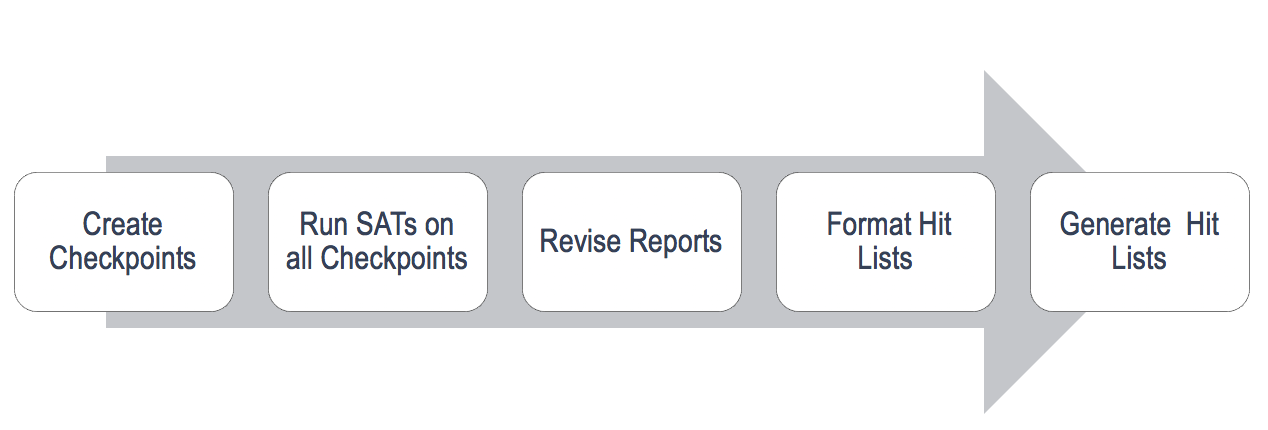
\includegraphics[height=1in, width=3in]{hit.png}
\caption{Steps that were conducted to generate hits lists reports}
\label{cyc}
\end{figure}

\begin{itemize}[leftmargin=*]
\item \textbf{ Step 1: Create Checkpoints}
The first task that we achieved is to create a list of candidate checkpoints for each repository. We fist dumped a list of commits dates for each repository. Then, we started from the date of the last commit and calculated the date differences of previous commits until we reached a commit with six month interval. Once we identify a commit with six months interval, we store both the commit hash (SHA value) and date. From the last stored commits that have six months interval we continue doing the same thing as we calculate the date difference with the remaining dates in the list until we reach the last date. By completing this step, we generating a list of \textbf{n} checkpoints for each repository depending on the age of that repository. Table \ref{stat} shows some statistics related to the project age (proj\_age) and number of checkpoints (n\_checkpnt) in our dataset.

\item \textbf{ Step 2: Run SATs on all Checkpoints}
Now each repository has a list of checkpoints. Hence in this step, we  run all static analysis tools (SATs) on all checkpoints of each tested repository.  So, when the analysis is run in a repository,  we first convert the working tree and the source code to match a given checkpoint (by performing subsequent \textbf{ git checkout commit-sha-value} on all considered checkpoint).  With each checkpoint we collected a number of metrics about that checkpoint, such as  number of source files (n\_src\_files), number of header files (n\_h\_files ), and line of codes (LOC) (See Table \ref{stat} for more information. We only considered the source and header files that are written in C++. So, we filtered the source files to only include files that have an extension of (C, cpp, CPP, cxx, cc, CC, cp, c++)  and header files that have an extension of(h, hh, hpp, H). This filtration also help us to direct static analysis tools to only analyze C++ files, as some of them (e.g., RATS) do multiple languages analysis. Indeed, our dataset includes projects that  include multiple programming languages, thus we wanted to restrict the analysis on C++ files only.

\item  \textbf{ Step 3: Revise Reports}
We revised all reports in terms of vulnerability type and tested file type. Regarding vulnerability type, each static analysis tool could detect different types of bugs. However, we only interested in buffer overflow vulnerabilities. Therefore, we had to provide a solution to only consider buffer overflow vulnerabilities. We goaled to do so with the initial analysis to reduce the required resources and the running time. Each tool was designed differently and generate the vulnerabilities in a variant way. Hence, we had to understand how these tools are generating their hit list in the first place.  Since, all studied tools are open source, that task was achievable. We found that Flawfinder includes 169 number of rules (primarily dangerous function names) in C/C++. Flawfinder allow users to specify which types of vulnerability to be analyzed. It is not obvious though, as Flawfinder does not declare that clearly.  However, by digging deeply into the source code, the documentation, and other files in Flawfinder package, we found a way of doing so. Flawfiner reports vulnerabilities based on the CWE/SANS top 25 list. It uses CWE identifiers to report any bug that matches the CWE pattern. For example, CWE-120 represents the classic buffer overflow vulnerability, which is copying the buffer without checking the size of the input. Thus, we used \textbf{--regex} flag to retrieve only CWE that are related to buffer overflow vulnerabilities. The CWE that we included are the following:


\begin{enumerate}
\item CWE-120: Classic buffer overflow 
\item CWE-126: Buffer Over-read
\item CWE-20: Improper Input Validation
\item CWE-119: Improper Restriction of Operations within the Bounds of a Memory Buffer
\item CWE-785: Use of Path Manipulation Function without Maximum-sized Buffer
\item CWE-676: Use of Potentially Dangerous Function
\end{enumerate} 

Other flags that used with Flawfinder are: \textbf{--quiet} to suppress all irrelevant information that are provided by the tool, such as which files are being analyzed while the tool is running. Also, we used \textbf{--context} flag to show which line of code that includes the vulnerability. This peace of information is very critical in our analysis, as most of the analyses depend primarily on it. In addition, we used \textbf{--dataonly} to obtain only the results and discard other information such as the headers and footers of the analysis. Finally, we used \textbf{--singleline} to show each bug report in single line, this would help us to create more neat hit list report.


With RATS, there is no way to specify which type of vulnerability to be analyzed. In fact, RATS uses different vulnerability database for each programming language. However, the tool provide a way to specify an alternate vulnerability database. So, we created our own vulnerability database that include buffer overflow vulnerabilities. In particular, we copied the original database and removed all other types of vulnerabilities other than buffer overflow vulnerabilities. We found that Rats includes 310 vulnerabilities reports, and only 213 for buffer errors.

When we run RATS, we use the flowing flags:  \textbf{-x} to avoid loading the default databases. Also, we used \textbf{-d} to load our alternate vulnerability database. 
In addition, we utilized  \textbf{--quiet} to suppress other ongoing irrelevant output, \textbf{ --resultsonly} to discard header, footer, and status information that are generated by default., and \textbf{---context} to show which line of code that include the vulnerability.

Cppcheck also could help to chose which bug report to be produced. The way that Cppchek does this is by allowing to suppress unwanted bug reports. It provide \textbf{--suppressions-list} flag and a user can generate a file that include unwanted bug warnings. We could get a list of all possible warnings in Cppcheck by running \textbf{--errorlist}. We found that Cppchek has 231 errors and only 31 are related to buffer overflow. So we created a list with 200 bug that should be suppressed.



We use a number of other Cppcheck flags as  well. We used \textbf{--quiet} to suppress all progress reports. Also, we used \textbf{ --language} flag to direct Cppcheck to check all files in the given language which is C++ in our case. In addition, \textbf{--template} was used to format the output report of the tool to be consistent with our report format. The following section include more information about our report format.  


Regarding the tested file type, we only interested in source code file that represents the program code and not source code files for test purposes. Therefore, in this step we removed all warnings that indicate that a given vulnerability happened in source code for test purposes. We inferred that from the file path which usually include any form of ``test'' keyword in it.
 
%"cppcheck:{file}:{line}:{severity}:{id}:{message}" 


\item \textbf{ Step 4: Format Hit Lists}
Each static analysis tool has its own format when it generates its hits list. When we analyzed a repository, we wanted to store all warnings of bugs at each checkpoint in one file.  Therefore, all warnings by all studied static analysis tools should be saved in one file to process them later. However, because our analysis depends mainly on processing these hit lists, we wanted to produce consistent and united format. This will make our analysis more easer and precise. Therefore, we generated our own formatted hits list as follow:
\newline

\fbox{\begin{minipage}{24em}
Tool Name : File Path : Line Number :Severity: Vulnerability Type : Context 
\end{minipage}}\\

By producing this kind of report, we insure that each bug warning has a its own signature.  \textbf{Tool Name} helps us to keep track which tool that produces such warning. This will help us to measure the precision and false positive rate for each tool.  \textbf{File Path} allow us to analysis and track the same file in different checkpoints in order to decide whether a given warning is false or true positive.  
\textbf{Line Number}  aids  us to insure that a given warning  is the same warning that appears in the same file but in other checkpoints. Also, sometime we could encounter situation where exact vulnerability that happen in the same file twice with different line numbers. Thus, line number would help us to differentiate between different vulnerabilities that hold the same context.  \textbf{Severity} this part of the report is generated by the studied static analysis tools by default. We thought that it could be beneficial to keep track of how the tool is evaluating a such  warning. Also, it could gives us more information when we extract the pattern of true positive warnings. Similarly \textbf{Vulnerability Type} also would aid us  to extract the pattern and the frequency of such vulnerability in real world. Finally  
\textbf{Context} is a very important element of the report. It could not only  help us to identify the uniqueness of the bug, but also it could serve  to reveal more information about the bug pattern, such as does it contains pointer operations?, what is the container of the bug?, what is the memory location?, etc.
 
 \item \textbf{ Step 5: Generate Hit Lists}
The last step was to generate hit lists of all static analysis tools against all studied repositories. All generated reports follow the format that was mentioned in Step 4.  Each repository includes \textbf{n} reports for each checkpoint.  We tested 40 repositories that include 341 checkpoints in total which means that we run all three static analysis tool 341 times. Also, in this step we collected some metrics about the warnings that were generated by each static analysis tool and the running times.
\begin{table}[ht]
\centering
\scriptsize
\caption{Summary statistics on the various metrics related to the studied static analysis tools.}
\label{SAT}
\begin{tabular}{||p{1.4cm}|p{.8cm} p{.7cm} p{.2cm} p{.7cm} p{.2cm} p{.5cm} p{.9cm}||}
\hline
\textbf{Statistic} & \textbf{Sum} & \textbf{Max} &	 \textbf{Min} 	& \textbf{Mean} 	&	 \textbf{Mode} 	& \textbf{Median} 	&  \textbf{Sst.Dev}\\
\hline\hline
RATS\_BO  & 47315 & 2582 &	0&	163.15	&0	&7&	406.73 \\
Flawfinder\_BO &96733 &3886 &	0 &	333.56 &	1	&16	&682.84 \\
Cppcheck\_BO &0 & 0	&0&	0	&0	&0	&0 \\

RATS\_rt & 264083 &12474&	15	&910.63&	104&	288.5	&1966.96\\

Falwfinder\_rt & 702497 &20014	&76&	2422.40&	588	&972.5&	4154.88 \\
Cppcheck\_rt &16551768 &2259102&	50	&57075.06&	58&	2089&	159674.17\\

\hline


\end{tabular}
\end{table}

Table \ref{SAT} shows some metrics regarding the detected vulnerabilities. These vulnerabilities are not unique meaning that one vulnerability could appear in different checkpoints, thus this table show the sum of all reported vulnerabilities. 
RATS\_rt , Falwfinder\_rt, and Cppcheck\_rt indicate the running time of each tool.  The running time in this table is measured in milliseconds. 





\end{itemize} 



%Then we build a tool that analyze these project by running open source static analysis tools that are shown in Table I. So, in general we will mainly use use source codes, commits, meta-data



\subsubsection{\textbf{Collecting Metrics Information}}
While we examined the studied repositories, we measured multiple metrics regarding the repositories to get better a better insight about our dataset. Table \ref{stat} shows some statistics related to the project age in months (proj\_age), number of commits (n\_commits),  number of checkpoints (n\_checkpnt),number of release (n\_release), number of the source files (n\_src\_files), number of header files (n\_h\_files), and line of code (LOC) of all studies repositories in our dataset. All statistics were collected using datamash tool \cite{datamash}.


\begin{table}[ht]
\centering
\scriptsize
\caption{Summary statistics on the various metrics related to the studied repositories.}
\label{stat}
\begin{tabular}{||p{1cm}|p{.5cm} p{.3cm} p{1cm} p{.6cm} p{.8cm} p{1cm}||}
\hline
\textbf{Statistic} & \textbf{Max} &	 \textbf{Min} 	& \textbf{Mean} 	&	 \textbf{Mode} 	& \textbf{Median} 	&  \textbf{Sst.Dev}\\
\hline\hline
proj\_age & 155 &	12	& 46.95	 & 12	& 35.5	& 31.1 \\                n\_commits & 8530	& 40& 	922.4	& 1651	& 392.5	& 1621.5 \\ 
n\_checkpnt & 42& 2	&8.5	&5&	6	&7.04  \\
n\_release &31	&0&	6.2	&0	&2.5 &	9.05  \\
n\_src\_files &899	&1	& 90.7 &	1 &38.5	&149.2 \\
n\_h\_files & 1017&	0&	122.4	&0	&52	& 212.7\\
LOC & 808325	& 5	&72831.3 &	90595	&23049.5&	143163.3  \\
\hline


\end{tabular}
\end{table}



%


\subsection{Analysis}
After the data collection phase, we got \textbf{n} number of hit lists in each repository based on the number of checkpoints for that repository. To answer each of our research questions, we needed to identify which vulnerability warning is false positive and which is true positive. Based on that information, we could get a list of true positive warnings that helps us to further answer RQ2 and RQ3. So, our method depend on analyzing vulnerabilities though history and based on that we could decide whether a given warnings is false or true positive. We have the following simple assumptions to decide if a warning is true or false positive:
\begin{enumerate}
\item False positive: we consider any warning that reappeared until the last updated check point as false positive. 
\item True positive: any vulnerability otherwise is considered to be true positive as it was removed in later versions. 
\end{enumerate}
\subsubsection{\textbf{Analysis Phases}}
Our data could be challenging, as we first need to know whether a vulnerability that appeared in checkpoint \textit{x} is the same exact one that appeared in checkpoint \textit{x+1}, etc. Some vulnerabilities could appear in one checkpoint and have the same exact signature but with different line number. Hence, with our analysis through the history we needed to know which one in checkpoint \textit{x} matches which one in checkpoint\textit{x+1}.
However, there could be a simpler situation where a vulnerability could reaper with the same whole exact signature. Thus, we wanted to do the analysis by initially excluding likely false positive warnings. So, we achieved the analysis in multiple phases. In the first phase,  we copied the hit list files that were generated initially to  edit them based on our finding on that phase. Then, we fed that particular phase files to the next phase to carry out 
the analysis on the next phase, and so on. All phases are illustrated in the following section:
\begin{itemize}

\item{\textbf{Phase one: exclude all likely false positive warnings}} In the first phase, all vulnerability warnings with the same exact signature (including the line number); that appeared at any checkpoint and still reappear continuously until the last checkpoint are considered to be false positives. We emphasis on the continuity of the warnings, as one warning that appears in  checkpoint \textit{x} then removed in checkpoint\textit{x+1}, but reappeared in checkpoint \textit{x+2} will not considered the same. In this situation we consider the warnings that appeared in checkpoint \textit{x} and checkpoint\textit{x+2} to be two different vulnerabilities. We did the analysis by examining the hit list of the last checkpoint with all previous checkpoints. In our analysis, we considered hit\_list\_1 to be the last updated one and hit\_list\_n to be the oldest hit list.
Hence, in this phase we fed copies of \textbf{n} hit list files of a repository that named as phase1\_hit\_list\_1 ... n to the analysis. Then, we just examine warnings that appeared in phase1\_hit\_list\_1 with all other previous n hit list files. When we found a warning that appeared exactly at all previous checkpoints continuously we marked it as false positive. For example, if we have 8 checkpoints, and thus we have files to be analyzed named as phase1\_hit\_list\_1 ... 8.  In this case we examine phase1\_hit\_list\_1 and all previous files. If we find for instance that  phase1\_hit\_list\_2 and phase1\_hit\_list\_3 have the same exact line of warnings we mark it as false positive. So we delete that line of warnings from phase1\_hit\_list\_1,2,3 and add that warning to a created \texttt{false\_positive} list. By doing so, we could feed phase1\_hit\_list1...n to the next phase and avoid analyzing the same warnings multiple times. Also, we could guarantee the uniqueness of the warning by counting all same false positive as one when store it in the false positive list. 


\item{\textbf{Phase two: exclude continuous false positive warnings}} in this phase we fed the phase1\_hit\_list1... n files that were generated in the previous phase into this phase and copied them to be named as  phase2\_hit\_list1... n. This will allow us to keep track of our data and keep as much as possible of information about the analysis. So, after excluding all false positives that have the same exact signature including the line number, we had to look for false positives that were still reintroduced in later versions until the last updated checkpoint. However this time we had to track potentially similar warnings but with different line numbers. First, we created a list of all possible exact warnings with different line number that appeared in the last updated checkpoint and among all checkpoints. So each warning is stored with all possible line numbers in other checkpoints. Note that some warnings could appears in checkpoint \textit{x} but in checkpoint \textit{x+1} there are two similar warnings both with different line number that the warning in checkpoint \textit{x}. So, we examined all warnings that appeared in phase2\_hit\_list1 and keep track of all previous and similar vulnerabilities in preceding checkpoints.  Then, we applied the \textbf{line\_match algorithm} which will be described in Section \ref{alg} to determine which vulnerabilities that match the last updated vulnerability. After that a list of all matching vulnerabilities in preceding checkpoints was created. So before we decide that a given vulnerability is false positive, we check to see whether the list that we got contain a contentious checkpoints. If that is the case, the vulnerability is considered as false positive, otherwise is left untouched. All false positives are deleted from phase2\_hit\_list\_1 and other hit lists that include the vulnerability, and added to the \texttt{false\_positive} list.


\item{\textbf{Phase three: exclude continuous true positive warnings}}
Similarly to previous phases, in this phase we fed the phase2\_hit\_list1... n files that were generated in the previous phase into this phase and copied them to be named as phase3\_hit\_list1... n. While, in all previous phases we only considered warnings that appeared in the last updated checkpoint and trace all similar vulnerabilities in preceding checkpoints, we considered all warnings that appeared at any checkpoint in this phase. That is because in the previous phases we were interested in all false positives, which imply that a vulnerability should appear in the last updated checkpoint to be considered false positive. However, in this phase we are interested in true positive that could appear any time. Actually in this phase phase2\_hit\_list1 should be empty as we had to remove all false positive warnings, and all we did in the previous phases is to remove other similar vulnerabilities from other checkpoints. In this phase, we loop through all checkpoints one by one and examined all warnings in that specific checkpoint with all previous checkpoints. We Started with phase3\_hit\_list\_2, because phase3\_hit\_list\_1 is already empty. Then when looped through all \textbf{n-2} previous checkpoints, then we examined phase3\_hit\_list\_3 with all previous checkpoints, and so on. With each loop, we created a list of potential  similar vulnerabilities in different checkpoints. Also, in this phase we used \textbf{line\_match algorithm}  to determine whether the given list of similar vulnerabilities with different line number in different checkpoints are indeed the same. The algorithm will produce a list of vulnerabilities that are the same with the matching checkpoint. So, similarly to phase 2 we check the continuity of the checkpoints. If a given list contains similar and continuous true positive warnings, the warnings are removed from the phase3\_hit\_list files and added to a created \texttt{true\_positive} list. Also, we extract the age of each true positive vulnerability and added to the \texttt{true\_positive} list. So, the \texttt{true\_positive} list contains the true positive warnings and the vulnerability age.


\item{\textbf{Phase four: exclude all remaining true positive warnings}}
Again, in this phase we fed the phase3\_hit\_list1... n files that were generated in the previous phase into this phase and copied them to be named as phase4\_hit\_list1... n. So, as we removed all false positive warnings and all continuous true positive warnings, the copied files will only include vulnerabilities that are unique and do not reintroduced in all other files ( and potentially all warnings that our algorithm failed to determine their continuity Section \ref{ttv}).  So, we looped through all phase4\_hit\_list files and stored the remaining warnings as true positives in the \texttt{true\_positive} list. When we added those vulnerabilities to the \texttt{true\_positive} list, we marked them as phase4 warnings and we did the same thing with phase3 warnings as well. This could help us with the further analyzing our algorithm.
\end{itemize}

\subsubsection{\textbf{line\_match Algorithm}\label{alg}}
Our problem requires to determine whether two  lines of code  in two different source code file versions are indeed the same. We first tried to use possible available git tools to do so. First, we thought of using \texttt{git blame}, however it does not really help with our problem as it does not tell if a given line of code is indeed the same in different versions of files. Also, \texttt{git diff} provide a general solution that only gives the number of added or deleted lines in examined files. Thus, we had to create our own solution which uses \texttt{git diff} that provides a partial solution. Therefore, we proposed this algorithm to enable us to trace and decide whether a given bug warning that appears in different versions of source code files is indeed the same. This algorithm could be also applied to any other problem where one needs to trace a line of code in different version of source code files. 

The main idea here is simply when  comparing two versions of files to trace a specific line, we want to to calculate the number of added and deleted lines up to that line number. To clarify this, let \texttt{a} be the first file to be compared and \texttt{b} be the second file to be fed to \texttt{git diff}.  Let \textit{l\_a} be the line of code that include the warning context in file \texttt{a} that is similar to \textit{l\_b} which is the line of code that include the warning context in file \texttt{b}. Also, let \textit{ln\_a} be the line number of \textit{l\_a} and  \textit{ln\_b} be the line number of \textit{l\_b}. 

%\begin{equation}
%\textit{l\_a} = \textit{l\_b} 
%\end{equation}
%\begin{equation}
%\textit{ln\_a} \neq \textit{ln\_b}
%\end{equation}

 
So, we want to see if these two lines  have different line numbers  due to file alteration. So by retrieving the original line number for both files and match each line number in file \textit{a} to the matching line number in  file \textit{b}. Then, when we counted the the number of addition and deletion until the line \textit{ln\_a}, so we could decide for sure if \textit{ln\_a} equal \textit{ln\_b}. However, how could we get this kind of information. Let first explain how \texttt{git diff} command output helped us. When issuing \texttt{git diff  commit\_a commit\_b filename}, the output gives a number of hunks that show one area where the files differ as follow:

@@ from-file-line-numbers to-file-line-numbers @@
The line numbers of the hunk usually look like ``start,count'' \texttt{start} refers to the line number that has changed, and \texttt{count} refers to how long the hunk is. When we specify \textbf{-U number}  flag (where \texttt{number} could include the maximum line number we could get), we could retrieve one hunk that includes the whole file from the beginning to the end.  Also, \texttt{git diff} prints \textbf{- , +} to indicate the addition or deletion of lines. So, by utilizing this information, we could retrieve line numbers in file \texttt{a} to match line numbers in file \texttt{b} based on the given hunk. Then, We could count the number of addition or deletion before and after \textit{ln\_a}.

%After that, we calculate the value \textit{alter\_diff} which refers to the difference between the addition and the deletion before \textit{ln\_a} as follow: 

% \begin{equation}
%\textit{alter\_diff} = \textit{num\_addition}  - \textit{num\_deletion} 
%\end{equation}

%Then, we calculated the difference between \textit{ln\_a} and \textit{ln\_b}

%\begin{equation}
%\textit{line\_diff} = \textit{ln\_b} - %\textit{ln\_a}
%\end{equation}

%If we find that \textit{line\_diff} = \textit{alter\_diff} this will indicate that the two lines are indeed the same.
Algorithm \ref{match}  shows the whole method.

 

\begin{algorithm}
 \KwData{ln\_b ,  ln\_a , filename, commit\_a , and commit\_b}
 \KwResult{ answer is ln\_b  equal  ln\_a} 

  git diff  -U max\_line\_num  commit\_a commit\_b  --  filename, then; 
  
  Using diff hunk, retrieve and match line numbers for files a and b; 
 
 Print all + and - marks and send the output to result\_file; 

num\_addition=0;

num\_deletion=0;

\While{reading result\_file}{
\While{ $line\_number <  $ln\_a}{
  read line\;
  \If{line \textbf{contains} + at the beginning}{
   num\_addition =  num\_addition + 1;  
   }
   
  
   \If{line \textbf{contains} - at the beginning}{
         num\_deletion =  num\_deletion + 1;    }
 
 }
 alter\_diff  =  num\_addition   -  num\_deletion;
 
 line\_diff  =  ln\_b  -  ln\_a;
 
 

\eIf{$alter\_diff =  $line\_diff }{
       $l\_a =  $l\_b;
   }
     { 
      $l\_a \neq $l\_b;
     }
 }
 
 
 
 \caption{ line\_match algorithm to determine whether two similar lines in two different versions of files are indeed the same}
 \label {match}
\end{algorithm}


To determine the altered lines of code, we use the algorithm to determine weather a line of code is related to addition and deletion in the other file version in the same hunk (in the same context by measure above and below code). Then, we use edit distance method to determine if the line is modified or not.
%\section{Results and Discussion}

\subsection{Static Analysis Tools Effectiveness}
In order to answer this question, we goaled to measure the effective of the studied static analysis tools in terms of precision, false positive rate, running time. We could not measure recall as we do not have all true vulnerabilities in advanced. We utilized the data that produced by our analysis to measure the Running time to measure how long it take one static analysis tool to analyze all studied repositories. In addition, we aimed to Precision and False positive rate as following: 

\begin{equation}
Precision = \frac  {\#TP}{\#TP + \#FP}
\end{equation}


\begin{equation}
False\_positive\_rate = \frac  {\#FP}{\#TP + \#FP}
\end{equation}


Regarding to the running time, as it is shown in Table \ref{SAT}, RATS consumed  264083 millisecond  which is 4.4747 minutes to finish analyzing 40 repositories with multiple checkpoints. Flawfinder took 702497 millisecond which means 11.708 minutes to achieve the same task. Although, Flawfinder generated larger number of warnings compared to RATS. Flawfinder has reported double warnings compared to RATS. Cppcheck consumed  4.597 hours to analyze 40 repositories, however, it did not report any buffer overflow vulnerability.  Table \ref{eff} shows the running time in minutes.



\begin{table}[ht]
\centering
\scriptsize
\caption{The effectiveness studied static analysis tools in terms of precision, false positive rate and runtime.}
\label{eff}
\begin{tabular}{||p{1cm}|p{2cm} p{2cm} p{2cm}||}
\hline
\textbf{Measure} & \textbf{RATS} &	 \textbf{Flawfinder} 	& \textbf{Cppceck} 	\\
\hline\hline
Precision & 0.357&0.537& NA\\
FP\_rate & 0.642 &0.462& NA\\
Runtime & 4.4 & 11.7 &275.8\\
\hline
\end{tabular}
\end{table}

As we can see from Table \ref{eff},  that Flawfinder is slightly more precise than RATS and has less false positive rate.  This could be interesting as Flawfinder produced more number of warnings as well. Hence, further analysis is required to determine where is the findings is true or this could happened due to another reason. Section \ref{ttv} includes more in information in this matter. Though, RATS runtime outperforms other tools. 



\subsection{True Positive Buffer Overflow Vulnerabilities Evolution}
In this section, we were interested in analyzing how did  true positive buffer overflow vulnerabilities evolved over time. In other words,  how long it took repository developers to  detect bugs then removed them from the repository. When we determined a such vulnerability as true positive,  we calculated its age by retrieving the date of the continuous checkpoints that appeared from the first appearance until the last checkpoint that was included. We computed the vulnerability age in month.  Figure~\ref{chart} shows the results obtained. We could see most of the true positives were detected in less than 6 month period of time. However, the chart also shows that there were some vulnerabilities that aged 71 months, about 5 years and 9 months, and then finally removed. In addition, we can see that there are spike at 13 months meaning there were also a number of vulnerabilities stayed undetected for around 2 years. Thus, we conclude that most of true positive are being removed in less than 6 month, however some of true positive vulnerabilities could stay for years without being removed. The result here could be related to the kind of static analysis tools that we studied ( string pattern matching) thus more advanced tools need to examined to reach to more robust conclusion.



\begin{figure} [h!]
\centering
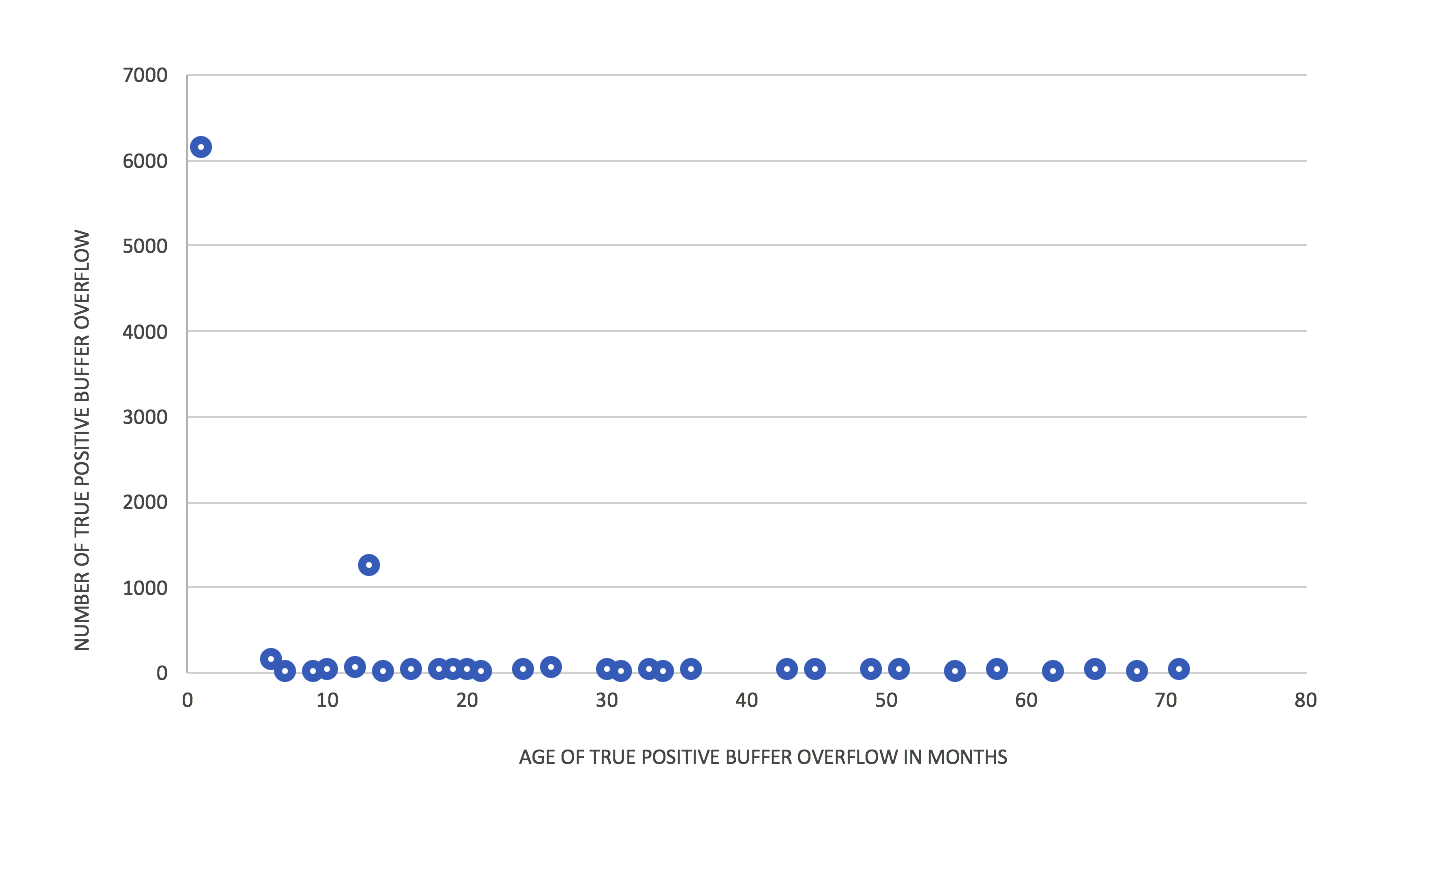
\includegraphics[height=2.5in, width=3.3in]{chart.png}
\caption{True positive buffer overflow vulnerabilities evolution over time}
\label{chart}
\end{figure}




\subsection{True Positive Buffer Overflow Vulnerabilities Patterns}

Finally, we wanted to study which kind of buffer overflow that were determined to be true positive and what pattern that it does hold. By examining all true positive warnings, we found 70 different kinds of warnings that occurred in true positive vulnerabilities. We divide these 70 warnings to three different  categories. The categories are as follow: (1) potentially dangerous function calls, (2) fixed buffer size, and (3) unsensitized input from untrusted source. Table \ref{patterns} shows our findings.




\begin{table}[ht]
\centering
\scriptsize
\caption{The percentages of true positive buffer overflow vulnerabilities patterns.}
\label{patterns}
\begin{tabular}{||p{5cm}|p{2cm} ||}
\hline
\textbf{Pattern} & \textbf{Percentages}  	\\
\hline\hline
Potentially dangerous function calls &  63\% \\
Fixed buffer size & 32\%  \\
Unsensitized input from untrusted source & 5\%\\
\hline
\end{tabular}
\end{table}

%\section{Threats to Validity \label{ttv}}
One possible threat to construct validity is the way that we run static analysis tools and the filtration to only include buffer overflow vulnerabilities. For example, in Flawfinder we included  CWE-20 that indicate ``Improper Input Validation'', which could include other types of vulnerabilities such as SQL injection. However, we further sanitized our hit lists to exclude all unrelated buffer overflow vulnerabilities from all the generated reports. Also,  we manually  analyzed some results to insure that we did not include any non relevant type of bugs. Another threats to construct validity is that our algorithm may not correctly decide a given vulnerability is indeed the same through the checkpoints. We manually analyzed randomly selected 20 vulnerabilities that span in multiple checkpoints in different 10 repositories. We found that it is always the case when the algorithm answers that a given vulnerability is the same through checkpoints, the answer is correct. For example, in some repositories we got a vulnerability line that happened in three different checkpoints . The three line number could have a difference of 300 lines, however the algorithm successfully determined that the line of the code is the same across the checkpoints. We found one  case that the algorithm rejected the matching and that was also correct answer. However, further investigation might be needed to include more cases to be manually  analyzed. 

One possible threat to internal validity could be the chosen number and type  repertoires. As the findings might be related to the very large size if repertoires, we might get different conclusion with small onces. In fact, even though we intended to study large program,  our dataset included  smaller once as well as it was shown in Table \ref{stat}. Also, as we analyzed only 40 repertoires we could not obtain  robust results. Therefore, we will improve our dataset in the future in terms of varying the repositories types and the size. Thus, in the future we will include 400 repositories that vary in size. Also, our analysis regrading false and true positives was mainly the removal of the code of line. However, that conclusion  might not be always true as the removed bug could be due to a change on the project design. Therefore, in the future we could apply more advanced techniques such as program slicing to get more solid conclusions. One threats to external validity is that we could not generalize our result to all other static analysis tools. However, we believe that our current algorithm could fit more advanced  static analysis tools.  In the future, we aim to include more advanced tools. 
 
%\section{Conclusion and Future Work}

 This work provides an evaluation of free and open source static analysis tools to detect buffer overflow. We used a different method than the traditional once to evaluation the static analysis tools. We mined real and large repositories to conduct the study. We designed an algorithm and created a tool for that algorithm, which could aid to trace one warnings though time. The algorithm run with large scale project with different commits to generate detect whether a buffer overflow warnings is true positive based on its history. 
 
In addition, we studied the age of the detected true positives and confirmed that most true positives are removed in less than 6 months. This study also gave us a better understanding about the pattern of buffer overflow bugs in which a static analysis tool able to detect. It implies that most buffer overflow true warnings occurred in potentially dangerous function calls.  In the future, we goal to study more advanced static analysis tools and improve the large and the quality of our dataset to produce more robust results. Also, we will improve our algorithm by including more semantic analysis. In addition, we might use the algorithm to  build a general tool that solve similar problems.   



\newpage
\bibliographystyle{IEEEtran}
\bibliography{bibliography}  
%\bibitem{IEEEhowto:kopka}
%H.~Kopka and P.~W. Daly, \emph{A Guide to {\LaTeX}}, 3rd~ed.\hskip 1em plus
% 0.5em minus 0.4em\relax Harlow, England: Addison-Wesley, 1999.

%\bibitem{lamport} L. Lamport, \emph{ {\LaTeX} A Document Preparation
%  System}, Reading, Mass: Addison-Wesley, 1994.

%\bibitem{knuth} D. E. Knuth, \emph {The \TeX book}, Reading, Mass.:
%  Addison-Wesley, 1996.


% that's all folks
\end{document}